\begin{refsection}

    \chapter[Insights from co-crystal structures]{New insights into chalcogen bonding provided by co-crystal structures of benzisoselenazolinone derivatives and nitrogen bases}\label{sec:crystengcomm1}
    
    This chapter was published in Cryst.\ Eng.\ Comm., 22 Jan 2019\autocite{Fellowes2019}.\footnote{Compound numbering, section headings, and terminology have been updated to fit this thesis.}
    
    \section{Abstract}
    A number of derivatives of benzisoselenazolinones, including the drug ebselen, have been synthesized, and their interactions with various nitrogen bases characterized through x-ray crystallography.
    Structural studies revealed a strong interaction in all cases, with \ce{Se \cdots N} distances well within the Van der Waals radii of the constituent atoms.
    We suggest that there is a significant charge transfer component to this interaction, in contrast to some other interactions of similar strength and directionality.
    We have also found that this interaction can be enhanced via H-bonding to the carbonyl group of the benzisoselenazolinone moiety.
    
    \cmpd*{ebs}
    \cmpd*{ebs.bn}
    \cmpd*{ebs.h}
    \cmpd*{amide}
    \cmpd*{amide.bn}
    \cmpd*{amide.h}
    \cmpd*{tetracycle}
    
    \section{Introduction}
    Chalcogen bonding (Ch-bonding) is a class of non-covalent interaction which has recently piqued the interests of the chemical community, and potential applications in materials and medicinal chemistry are emerging.\autocite{Mitchell2017,Wonner2017a,Fanfrlik2014,Vogel2019}
    It bears similarities to the related concept of halogen bonding, and the ubiquitous phenomenon of hydrogen bonding, in that the result is a relatively strong and highly directional non-bonded interaction.\autocite{Paolo1974}
    This strength and directionality has been exploited in crystal engineering\autocite{Gleiter2003,Kremer2016,Huynh2017}, anion recognition\autocite{Lim2017,Lim2018,Garrett2016}, and bond activation \autocite{Wonner2017,Benz2017,Benz2017a}, and appears to play a critical role in protein folding.\autocite{Iwaoka2001,Iwaoka2015}
    Studies on \ce{Te \cdots N} Ch-bonds in solution phase have shown they can be as strong as 2.7~kcal/mol\autocite{Garrett2015a}.
    A number of interesting and potentially useful supramolecular polymers have been synthesised and characterised by \citeauthor{Ho2016,Ho2017}, based on tellurium- and selenium-containing heterocycles.\autocite{Ho2016,Ho2017}
    
    In our efforts to apply the concept of Ch-bonding to biological systems, we turned to the benzisoselenazolinone scaffold of the antioxidant compound ebselen \cmpd{ebs}.
    \cmpd{ebs} has been known since the 1980s to effectively scavenge reactive oxygen species \emph{in vivo}.\autocite{Muller1984}
    It has remarkably low toxicity for an organoselenium compound, and is being investigated as a possible treatment for a number of conditions.\autocite{Schewe1995,Kil2007,Singh2013,Parnham2000}
    It is also an ideal scaffold for Ch-bonding, bearing a selenium atom bonded to an electronegative amide nitrogen.
    Indeed, Ch-bonding in \cmpd{ebs} has been investigated previously in the context of crystal packing of the pure compound, but there is a lack of experimental evidence for interactions with other acceptors.\autocite{Thomas2015}
    
    Numerous studies have examined the nature of the Ch-bond, in particular the balance between electrostatic effects (due to anisotropic electrostatic potential around the chalcogen atom), covalent (orbital overlap and electron delocalisation), and dispersion forces.\autocite{Oliveira2017,Pascoe2017,DeVleeschouwer2017,Kolar2016,Gleiter2018}
    In the case of halogen bonding, these contributions are generally well characterized.
    Halogen bonds range from primarily electrostatic (as in the case of fluorinated iodobenzenes\autocite{Prasang2009}) to charge-transfer dominated (molecular halogens\autocite{Mulliken1950}).
    In the case of Ch-bonding in derivatives of \cmpd{ebs}, the contributions are less clear.
    We therefore sought to characterize Ch-bonding interactions between a number of derivatives of \cmpd{ebs}, and a variety of Ch-bond acceptors.
    
    
    \section{Results and Discussion}
    \subsection[Synthesis of \refcmpd{ebs,ebs.bn,tetracycle}]{Synthesis of benzisoselenazolinone derivatives \refcmpd{ebs,ebs.bn,tetracycle}}
    Compounds \cmpd{ebs} and \cmpd{ebs.bn} were synthesized via published procedures from amides \cmpd{amide} and \cmpd{amide.bn}.\autocite{Bhabak2010}
    The Se-tetracycle \cmpd{tetracycle} was isolated in poor yield as the major product from the cyclization of primary amide \cmpd{amide.h} in an attempt to form \cmpd{ebs.h}.
    It is noteworthy that the spectral characteristics of \cmpd{tetracycle} are essentially identical to reported spectral data of \cmpd{ebs.h}\autocite{Bhabak2010}.
    
    \begin{scheme}
      \centering
      \replacecmpd{amide,amide.bn}
      \replacecmpd{ebs,ebs.bn}
      \replacecmpd{amide.h}
      \replacecmpd{ebs.h}
      \replacecmpd{tetracycle}
      \replacecmpd{ebs}
      \replacecmpd{ebs.bn}
      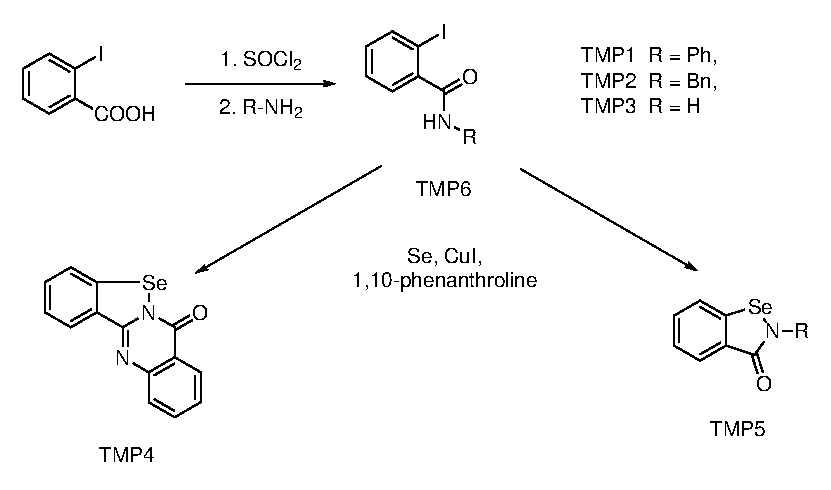
\includegraphics[scale=0.74]{Figures/catalytic-synthesis.eps}
      \caption{Synthesis of Ch-bond donors \refcmpd{ebs}, \refcmpd{ebs.bn} and \refcmpd{tetracycle}.}\label{fig:synthesis}
    \end{scheme}
    
    \begin{table}
      \centering
      \caption{Selected structural parameters of Ch-bonded complexes.}\label{tab:bondlengths}
      \tablefit{\begin{tabular}{lllllll}
        \toprule
        Complex & r(\ce{N \cdots Se}) & r(\ce{Se-N_{1}}) & r(\ce{Se-C_{1}}) & r(\ce{N-C(O)}) & $ \angle $(\ce{N \cdots Se-N_{1}}) & $ \angle $(\ce{C_{para} \cdots N \cdots Se}) \\
          & \AA\ & \AA\ & \AA\ & \AA\ & \degree\ & \degree\  \\ \midrule
        \cmpd{ebs} only & --- \\
        \cmpd{ebs} $ \cdot $ DMAP & 2.371(1) & 1.9676(10) & 1.8959(12) & 1.2345(14) & 174.18(4) & 173.52(4) \\
        \cmpd{ebs.bn} only & --- & 1.8805(14) & 1.8867(16) & 1.350(2) & --- & --- \\
        \cmpd{ebs.bn} $ \cdot $ DMAP M1 & 2.4276(14) & 1.9297(13) & 1.8984(15) & 1.348(2) & 173.93(5) & 174.89(5) \\
        \cmpd{ebs.bn} $ \cdot $ DMAP M2 & 2.4331(14) & 1.9191(14) & 1.8966(14) & 1.349(2) & 175.30(5) & 158.14(5) \\
        \cmpd{ebs.bn} $ \cdot $ DMAP $ \cdot $ \ce{H2O} & 2.4046(15) & 1.9367(14) & 1.9070(14) & 1.330(2) & 175.54(5) & 167.43(5) \\
        \cmpd{ebs.bn} $ \cdot $ quinuclidine & 2.5874(17) & 1.9077(17) & 1.898(2) & 1.354(3) & 176.77(7) & 161.32(7) \\
        \cmpd{ebs.bn} $ \cdot $ DABCO & 2.6166(15) & 1.9019(14) & 1.8967(17) & 1.355(2) & 175.76(6) & 160.00(6) \\
        \cmpd{tetracycle} only & --- & 1.883(2) & 1.899(3) & 1.393(3) & --- & --- \\
        \cmpd{tetracycle} $ \cdot $ pyridine & 2.461(3) & 1.926(2) & 1.908(3) & 1.373(4) & 174.13(9) & 169.1(1)\\
        \cmpd{tetracycle} $ \cdot $ DMAP & 2.304(1) & 1.9716(9) & 1.918(1) & 1.375(1) & 173.81(4) & 173.16(4) \\
        \bottomrule
        \end{tabular}}
    \end{table}
    
    \subsection{Co-crystal structures of benzisoselenazolinones and Lewis bases}
    High quality low temperature crystal structures were obtained for the parent benzisoselenazolinone derivatives \cmpd{ebs} \autocite{Thomas2015}, \cmpd{ebs.bn} and the Se-tetracycle \cmpd{tetracycle} and the chalcogen-bonded co-crystals of these compounds with a variety of nitrogen bases, including pyridine, dimethylaminopyridine (DMAP), quinuclidine and 1,4-diaza\-bicyclo[2.2.2]\-octane (DABCO).
    Powder diffraction patterns were obtained of the bulk co-crystal material and compared with the single crystal data, with excellent agreement.
    This provides strong evidence of phase purity, with the exception of \cmpd{ebs.bn}$ \cdot $DMAP, which indicated the presence of the unbound monomers in addition to the Ch-bonded adduct.
    Relevant structural parameters are presented in \cref{tab:bondlengths}, while all thermal ellipsoid plots are presented in the supplementary material (\cref{sec:ch3-si}).
    In the following discussion we begin by assessing the Ch-bond donor abilities of \cmpd{ebs}, \cmpd{ebs.bn}, and \cmpd{tetracycle} by comparing the structural parameters with a common nitrogen base adduct (DMAP), followed by comparison of a single Ch-bond donor \cmpd{tetracycle} with two different nitrogen bases with markedly different basicities (pyridine and DMAP).
    
    \subsection{Effects of the benzisoselenazolinone on Ch-bond strength}
    The DMAP adducts of \cmpd{ebs}, \cmpd{ebs.bn} and \cmpd{tetracycle} are characterized by near linear \ce{N \cdots Se-N(CO)} angles (\cref{tab:bondlengths}) with \ce{N_{DMAP} \cdots Se}distances which are 2.4276(14) and 2.4331(16)~\AA\ for the two independent molecules of \cmpd{ebs.bn}, 2.371(1)~\AA\ for \cmpd{ebs}, and the strikingly short \ce{N \cdots Se} distance of 2.304(1)~\AA\ for \cmpd{tetracycle}.
    All are well within the van der Waals radii of N and Se of 3.85~\AA\ \autocite{Batsanov2001}.
    The antipodal \ce{Se-N_{1}} bond distance within these adducts is significantly lengthened compared to the free Ch-bond donors, 0.063~\AA\ in \cmpd{ebs}, 0.049~\AA\ in \cmpd{ebs.bn}, and 0.088~\AA\ in \cmpd{tetracycle}, with the degree of lengthening being related in an inverse sense to the \ce{N_{DMAP} \cdots Se}distance, in all cases the (non-antipodal) \ce{Se-C_{1}} bond is essentially unchanged.
    These structural parameters suggest an order of Ch-bond donor abilities \cmpd{ebs.bn} < \cmpd{ebs} < \cmpd{tetracycle}, which is supported by theoretical calculations which are discussed below, as well as being consistent with the \textsuperscript{77}Se NMR chemical shifts.
    
    \subsection{Endocyclic bond lengthening associated with stronger complexes}
    Further discussion is warranted on the \cmpd{ebs.bn}$ \cdot $DMAP adduct.
    Firstly, the two independent molecules of \cmpd{ebs.bn}$ \cdot $DMAP differ significantly with respect to the direction that the nitrogen base lone pair makes with the \ce{Se-N_{1}} bond.
    In molecule 1 this angle is close to collinear at 174.89(5)\degree\ while in molecule 2, this deviates significantly from linearity 158.14(5)\degree.
    Associated with this difference is a slightly longer \ce{N_{DMAP} \cdots Se} distance of 2.4331(14)~\AA\ in molecule 2 compared to 2.4276(14)~\AA\ in molecule 1 ($ \Delta $=0.0055~\AA{}; 3$ \sigma $) and a shorter \ce{Se-N_{1}} distance 1.9191(14)~\AA\ vs 1.9297(14)~\AA\ ($ \Delta $=-0.10~\AA{}; 7.5$ \sigma $) indicating a slightly weaker interaction.
    This can be seen in \cref{fig:benzyl-dmap-xray-2}.
    
    \begin{figure}
      \centering
      \includegraphics[width=0.8\linewidth]{Figures/benzyl-dmap-xray-2.pdf}
      \caption{Structure of \refcmpd{ebs.bn}$ \cdot $DMAP, showing the two distinct geometries.}\label{fig:benzyl-dmap-xray-2}
    \end{figure}
    
    The structural effects described, particularly the lengthening of the \ce{Se-N_{1}} bond are consistent with donation of electron density from the nitrogen lone pair into the \ce{Se-N_{1}} anti-bonding orbital being a significant component of these \ce{N \cdots Se} Ch-bonds, which has been described before\autocite{Pascoe2017}.
    
    \subsection{H-bond enhanced Ch-bonding}
    The second reason for further discussion of the \cmpd{ebs.bn}$ \cdot $DMAP adduct is based on the structural parameters obtained for the hydrate structure \cmpd{ebs.bn}$ \cdot $DMAP$ \cdot $\ce{H2O} which was serendipitously obtained by evaporation of a THF solution in an open flask.
    The structure is shown in \cref{fig:benzyl-dmap-hydrate}.
    
    \begin{figure}
      \centering
      \includegraphics[width=0.8\linewidth]{Figures/benzyl-dmap-hydrate.pdf}
      \caption{Structure of \refcmpd{ebs.bn}$ \cdot $DMAP$ \cdot $\ce{H2O}.}\label{fig:benzyl-dmap-hydrate}
    \end{figure}
    
    \cmpd{ebs.bn}$ \cdot $DMAP$ \cdot $\ce{H2O} crystallizes as a centrosymmetric hydrogen-bonded dimer in which two water molecules bridge two molecules of \cmpd{ebs.bn} across a crystallographic inversion centre.
    Of note, when comparison is made between the structural parameters for \cmpd{ebs.bn}$ \cdot $DMAP molecule 1, which has a similar geometry about the \ce{N \cdots Se} moiety as for \cmpd{ebs.bn}$ \cdot $DMAP$ \cdot $\ce{H2O}, there is a significant contraction of the \ce{N_{DMAP} \cdots Se}distance from 2.4276(14)~\AA\ to 2.4046(14)~\AA\ ($ \Delta $=-0.023~\AA{}; 16$ \sigma $), and an increase in the \ce{Se-N_{1}} bond distance from 1.9297(13) to 1.9367(14)~\AA\ ($ \Delta $=0.007~\AA{}; 5$ \sigma $).
    We have coined the term `hydrogen-bond enhanced Ch-bonding' to describe this interesting structural effect.
    
    \subsection{Effects of the Lewis base on Ch-bond strength}
    We were fortunate to obtain crystal structures of the Se-tetracycle \cmpd{tetracycle} with both pyridine and DMAP, which gave us the opportunity to compare the structural effects arising from two Ch-bond acceptors with significantly different basicities.
    The pyridine adduct of \cmpd{tetracycle} is characterized by a \ce{N_{PYR} \cdots Se} distance 2.461(3)~\AA\ and \ce{Se-N_{1}} distance of 1.926(2)~\AA\ and a near linear \ce{N_{PYR} \cdots Se-N_{1}} angle, the \ce{Se-N_{1}} bond distance is significantly longer than the corresponding distance 1.883(2)~\AA\ in non-bound structure of \cmpd{tetracycle}.
    The DMAP adduct of \cmpd{tetracycle} is characterized by a significantly shorter \ce{N_{DMAP} \cdots Se} distance of 2.304(1)~\AA\ ($ \Delta $=-0.157~\AA) and longer \ce{Se-N_{1}} distance of 1.9716(9)~\AA\ ($ \Delta $=0.046~\AA), consistent with a significantly stronger interaction.
    
    \begin{figure}
      \centering
      \includegraphics[width=0.8\linewidth]{Figures/dimer-dmap-py-xray.pdf}
      \caption{Pyridine and DMAP adducts of Se-tetracycle \refcmpd{tetracycle}.}\label{fig:dimer-adducts}
    \end{figure}
    
    Ch-bonded co-crystals of the benzisoselenazolinone derivative \cmpd{ebs.bn} with the tertiary amines; quinuclidine and DABCO were obtained and structurally characterized.
    The adducts are presented in \cref{fig:benzyl-adducts}.
    The \ce{N_{QUIN} \cdots Se} and \ce{N_{DABCO} \cdots Se} distances of 2.5874(17)~\AA\ and 2.6166(15)~\AA\ for \cmpd{ebs.bn}$ \cdot $quinuclidine and \cmpd{ebs.bn}$ \cdot $DABCO respectively are significantly longer than those observed for \cmpd{ebs.bn}$ \cdot $DMAP suggesting an order of Ch-bond strengths with \cmpd{ebs.bn} DABCO < Quinuclidine < DMAP which correlates well with the hydrogen bond acceptor ability of these bases, as quantified by the pK\textsubscript{HB} (\cref{tab:pkhb}).
    
    \begin{table}
      \centering
      \caption{Hydrogen bond basicities of bases studied.}\label{tab:pkhb}
      \begin{tabular}{lllll}
        \toprule
                                & pyridine                      & DABCO                     & quinuclidine              & DMAP \\\midrule
          pK\textsubscript{HB}  & 1.86\autocite{Berthelot1998}  & 2.63\autocite{Graton2002} & 2.71\autocite{Graton2002} & 2.80\autocite{Berthelot1998}\\
          \cmpd{ebs.bn}$ \cdot $base r(\ce{N \cdots Se}) / \AA\ & ---   & 2.6166(15)                & 2.5874(17)                & 2.4276(14)\footnote{Bond distance given is the shorter of the two coordination environments.}\\
          \cmpd{ebs.bn}$ \cdot $base $ \Delta $H\textsubscript{f} / kcal/mol & -6.35    & -7.82 & ---                       & -7.91\\\bottomrule
      \end{tabular}
    \end{table}
    
    \begin{figure}
      \centering
      \includegraphics[width=0.8\linewidth]{Figures/benzyl-quin-dabco-xray.pdf}
      \caption{Adducts of benzisoselenazolinone \refcmpd{ebs.bn} with quinuclidine and DABCO.}\label{fig:benzyl-adducts}
    \end{figure}
    
    \subsection{DFT interaction energies and NBO analysis}
    Interaction energies for the complexes were calculated using the $ \omega $B97X-D dispersion corrected functional, which has been used to study similar systems with good agreement with coupled cluster methods.\autocite{Oliveira2017}
    All geometries were therefore optimized at $ \omega $B97X-D/def2-TZVP, and minima verified by frequency analysis.
    
    \begin{figure}
      \centering
      \includegraphics[width=0.8\linewidth]{Figures/dft-energies.pdf}
      \caption[Interaction energies for various complexes.]{Interaction enthalpies calculated at $ \omega $B97X-D/def2-TZVP.\@ Optimised geometries for the DMAP complexes are shown to the left.}
    \end{figure}
    
    NBO analysis was conducted on the optimized geometries, which supports our suggestion that there is a strong orbital component to Ch-bonding in these systems.
    Second order perturbation theory revealed that the energy associated with n(N\textsubscript{base})$ \rightarrow $ $ \sigma^{\star} $(N\textsubscript{1}--Se) delocalisation was 12.79, 15.45, and 16.23~kcal/mol for \cmpd{ebs.bn}$ \cdot $DMAP, \cmpd{ebs}$ \cdot $DMAP, and \cmpd{tetracycle}$ \cdot $DMAP respectively.
    %In the case of the \cmpd{ebs.bn}$ \cdot $DMAP$ \cdot $\ce{H2O} complex, the delocalisation energy was 13.51~kcal/mol.
    %This consistent with our experimental observation of hydrogen-bond enhanced Ch-bonding.
    
    \begin{figure}
      \centering
      \includegraphics[width=0.6\linewidth]{Figures/phenyl-dmap-overlap.pdf}
      \caption[Orbital overlap for \refcmpd{ebs}$ \cdot $DMAP.]{Overlap of nitrogen lone pair with $ \sigma^{\star} $(\ce{Se-N}) in \refcmpd{ebs}$ \cdot $DMAP complex.}\label{fig:phenyl-dmap-overlap}
    \end{figure}
    
    \section{Conclusion}
    In summary, we have demonstrated the importance of Ch-bonding between derivatives of ebselen \cmpd{ebs} and a variety of nitrogen bases.
    These selenium-containing heterocycles form close contacts with electron pair donors, well within the Van der Waals radii, with predictable geometries consistent with the Ch-bonding model.
    These interactions appear to be primarily due to orbital overlap as opposed to electrostatic or dispersion mediated effects, as evidenced by lengthening of the antipodal \ce{Se-N} bond, and computational analysis, which is consistent with findings in related systems by \citeauthor{Pascoe2017}.\autocite{Pascoe2017}
    We have also found that the strength of a Ch-bond can be enhanced via a hydrogen bond to the carbonyl group of the heterocycle.
    We hope to exploit the strength and directionality of Ch-bonds in ebselen to target biomolecules such as nucleic acids and proteins using compounds containing the isoselenazolinone moiety.
    
    \section{Supplementary materials}
    
    \subsection{Synthetic procedures}
    
    \subsubsection[Preparation of \refcmpd{ebs}.]{Preparation of 2-phenylbenzo[\textit{d}][1,2]selenazol-3(2\textit{H})-one \refcmpd{ebs}.}
    
    Copper iodide (98.4~mg, 0.517~mmol) and 1,10-phenanthroline (83.1~mg, 0.461~mmol) were stirred in anhydrous DMF (3~mL) for 15 mins at r.t., then 2-iodo-N-phenylbenz\-amide (653.2~mg, 2.021~mmol), selenium (196.9~mg, 2.495~mmol) and potassium carbonate (627.3~mg, 4.539~mmol) were added sequentially under a flow of argon.
    The mixture was heated at 110\degree{}C for 8~h, when TLC showed consumption of starting material.
    The mixture was then tipped into brine (30~mL) and stirred to form a brown precipitate, which was extracted into DCM (40~mL) and washed with water ($ 2 \times 20 $~mL).
    The DCM solution was filtered through a silica plug, then evaporated, and the residue applied to a SNAP 25~g silica cartridge, eluting with a petroleum ether/ethyl acetate gradient.
    The major peak was evaporated to afford colourless crystals of \cmpd{ebs} (378.8~mg, 69\%, m.p. 179.1--180.3\degree{}C, lit.\ mp 180--181\degree{}C). 
    
    \ce{^{1}H} NMR (499~MHz, \ce{\textit{d}6}-DMSO) $ \delta $ ppm 8.07 (1H, d, \textit{J} = 8.02~Hz), 7.90 (1H, d, \textit{J} = 7.45~Hz), 7.68 (1H, t, \textit{J} = 7.25~Hz), 7.61 (2H, d, \textit{J} = 7.68~Hz), 7.52--7.42 (3H, m), 7.26 (1H, t, \textit{J} = 7.39~Hz).
    
    \ce{^{77}Se} NMR (95~MHz, \ce{\textit{d}6}-DMSO) $ \delta $ 959.66.
    
    \subsubsection[Preparation of \refcmpd{ebs.bn}.]{Preparation of 2-benzylbenzo[\textit{d}][1,2]selenazol-3(2\textit{H})-one \refcmpd{ebs.bn}.}
    
    Copper iodide (95.8~mg, 0.503~mmol) and 1,10-phenanthroline (93.8~mg, 0.521~mmol) were stirred in anhydrous DMF (3~mL) for 15 mins at r.t., then N-benzyl-2-iodobenz\-amide (860.9~mg, 2.553~mmol), selenium (256.6~mg, 3.249~mmol) and potassium carbonate (542.2~mg, 3.923~mmol) were added sequentially under a flow of argon.
    The mixture was heated at 110\degree{}C for 5~h, when TLC showed consumption of starting material.
    The mixture was then tipped into brine (30~mL) and stirred to form a solid mass, which was dissolved in DCM (40~mL) and washed with water ($ 2 \times 20 $~mL).
    The DCM solution was filtered through a silica plug, then evaporated, and the residue applied to a SNAP 50~g silica cartridge, eluting with a petroleum ether/ethyl acetate gradient.
    The major peak was evaporated to afford pale yellow crystals of \cmpd{ebs.bn} (396.4~mg, 53\%, m.p. 137.8--138.8\degree{}C).
    
    \ce{^{1}H} NMR (400~MHz, \ce{\textit{d}6}-DMSO) $\delta$ ppm 7.99 (1H, d, \textit{J} = 8.04~Hz), 7.83 (1H, d, \textit{J} = 7.7~Hz), 7.59 (1H, t, \textit{J} = 7.56~Hz), 7.42 (1H, t, \textit{J} = 7.44~Hz), 7.37--7.22 (5H, m), 4.9 (2H, s).
    
    \ce{^{77}Se} NMR (95~MHz, \ce{\textit{d}6}-DMSO) $ \delta $ 884.02.
    
    \subsubsection[Preparation of \refcmpd{tetracycle}.]{Preparation of 5\textit{H}-benzo[4,5][1,2]selenazolo[2,3-\textit{a}]quinazolin-5-one \refcmpd{tetracycle}.}
    
    Copper iodide (96.4~mg, 0.503~mmol) and 1,10-phenanthroline (85.7~mg, 0.476~mmol) were stirred in anhydrous DMF (4~mL) for 10~mins at r.t., then 2-iodobenzamide (510.6~mg, 2.067~mmol), selenium (209.5~mg, 2.653~mmol) and potassium carbonate (506.3~mg, 3.663~mmol) were added sequentially under a flow of argon.
    The mixture was heated at 110\degree{}C for 12~h, when TLC showed consumption of starting material.
    The mixture was then tipped into brine (30~mL) and stirred to form a solid mass, which was extracted into ethyl acetate (20~mL) and washed with water ($ 2 \times 20 $~mL).
    The DCM solution was filtered through a silica plug, then evaporated, and the residue applied to a SNAP 50~g silica cartridge, eluting with a petroleum ether/ethyl acetate gradient.
    The major peak was evaporated to afford pale yellow crystals of \cmpd{tetracycle} (45.8~mg, 15\%, m.p. 267--268\degree{}C). 
    
    \ce{^{1}H} NMR (499~MHz, \ce{CDCl3}) $\delta$ ppm 8.49 (1H, d, \textit{J} = 7.92~Hz), 8.39 (1H, dd, \textit{J}\textsubscript{1} = 1.05~Hz, \textit{J}\textsubscript{2} = 8.01~Hz), 7.91 (1H, d, \textit{J} = 7.85~Hz), 7.88--7.84 (1H, m), 7.8 (1H, d, \textit{J} = 7.98~Hz), 7.76--7.7 (1H, m), 7.63--7.54 (2H, m).
    
    \ce{^{77}Se} NMR (95~MHz, \ce{CDCl3}) $ \delta $ 992.48.
    
    \subsection{Crystallographic data}\label{sec:ch3-si}
    Intensity data was collected on an Oxford Diffraction SuperNova CCD diffractometer using either Cu-K$\alpha$ or Mo-K$\alpha$ radiation at 130.0(1)~K, or on a Rigaku XtalLAB Synergy at 100.0(1)~K. Compound \cmpd{ebs.bn}$ \cdot $DMAP$ \cdot $\ce{H2O} underwent a destructive phase change when cooling to 130~K, therefore data were collected at 200~K. Data for \cmpd{tetracycle} was collected on the MX1 beam line at the Australian Synchrotron\autocite{Cowieson2015}. The temperature was maintained using an Oxford Cryostream cooling device. The structures were solved by direct methods and difference Fourier synthesis.\autocite{Sheldrick2015} Thermal ellipsoid plot was generated using the program ORTEP-3\autocite{Farrugia1997} integrated within the WINGX\autocite{Farrugia1999} suite of programs.
    
    \subsubsection{Crystal data for \texorpdfstring{\refcmpd{ebs}$ \cdot $DMAP}{C20H19N3OSe}}
    \ce{C20H19N3OSe}, $M=396.34$, $T=130.0$~K, $ \lambda=0.71073 $~\AA, Triclinic, space group P$\bar{1}$, $a = 8.3674(3)$, $b = 9.8399(5)$, $c =10.6622(5)$~\AA, $\alpha=93.296(4)$\degree, $\beta=93.021(4)$\degree, $\gamma=101.210(4)$\degree, $V=857.86(7)$~\AA$^{3}$, $Z = 2$.
    $D_{c}= 1.534$~mg~M$^{-3}$, $\mu$(Mo-K$\alpha$) = 2.201~mm$^{-1}$, F(000) = 404, crystal size $0.52 \times 0.34 \times 0.23$~mm.
    11339 reflections measured, $\theta_{\max}=36.66$\degree, 7889 independent reflections, R\textsubscript{int} = 0.0163, the final R was 0.0293 ($I > 2\theta(I)$, 6882 reflections) and \textit{w}R(F\textsuperscript{2}) was 0.0721 (all data), GOF 0.992.
    CCDC 1867205.
    From dichloromethane/pentane (70\%) m.p. 111.3--112.1\degree{}C.
    
    \begin{figure}
      \includegraphics[width=0.6\linewidth]{Figures/ebs-dmap-xtal.pdf}
      \caption{X-ray crystal structure of \texorpdfstring{\refcmpd{ebs}$ \cdot $DMAP}{C20H19N3OSe}.}
    \end{figure}
    
    \subsubsection{Crystal data for \texorpdfstring{\refcmpd{ebs.bn}}{C14H11NOSe}}
    \ce{C14H11NOSe}, $M=288.20$, $T=100.0$~K, $ \lambda=0.71073 $~\AA, Orthorhombic, space group Pca2\textsubscript{1}, $a = 11.7848(3)$, $b = 4.5869(1)$, $c = 21.3572(5)$~\AA, $V = 1154.48(5)$~\AA$^{3}$, $Z = 4$.
    $D_{c}= 1.658$~mg~M$^{-3}$, $\mu$(Mo-K$\alpha$) = 3.233~mm$^{-1}$, F(000) = 576, crystal size $0.63 \times 0.54 \times 0.22$~mm.
    44918 reflections measured, $\theta_{\max}=45.38$\degree, 9588 independent reflections, R\textsubscript{int} = 0.0481, the final R was 0.0331 ($I > 2\theta(I)$, 7848 reflections) and \textit{w}R(F\textsuperscript{2}) was 0.0792 (all data), GOF 1.063.
    CCDC 1867211.
    
    \begin{figure}
      \includegraphics[width=0.6\linewidth]{Figures/ebs-bn-xtal.pdf}
      \caption{X-ray crystal structure of \texorpdfstring{\refcmpd{ebs.bn}}{C14H11NOSe}.}
    \end{figure}
    
    \subsubsection{Crystal data for \texorpdfstring{\refcmpd{ebs.bn}$ \cdot $DMAP$ \cdot $\ce{H2O}}{C21H21N3OSe.(H2O)}}
    \ce{C21H21N3OSe.(H2O)}, $M=428.38$, $T=200.0$~K, $ \lambda=0.71073 $~\AA, Triclinic, space group P$\bar{1}$, $a = 9.6254(2)$, $b = 10.2486(2)$, $c = 10.6505(2)$~\AA, $\alpha = 83.660(2)$\degree, $\beta = 76.398(2)$\degree, $\gamma = 78.423(2)$\degree, $V = 998.19(4)$~\AA$^{3}$, $Z = 2$.
    $D_{c}= 125$~mg~M$^{-3}$, $\mu$(Mo-K$\alpha$) = 1.901~mm$^{-1}$, F(000) = 440, crystal size $0.41 \times 0.32 \times 0.23$~mm.
    30047 reflections measured, $\theta_{\max} = 41.06$\degree, 12528 independent reflections, R\textsubscript{int} = 0.0267, the final R was 0.0456 ($I > 2\theta(I)$, 6303 reflections) and \textit{w}R(F\textsuperscript{2}) was 0.1219 (all data), GOF 1.000.
    CCDC 1867213.
    From THF in an open flask (90\%) m.p. 96--97\degree{}C.
    
    \begin{figure}
      \includegraphics[width=0.6\linewidth]{Figures/ebs-bn-dmap-hydrate-xtal.pdf}
      \caption{X-ray crystal structure of \texorpdfstring{\refcmpd{ebs.bn}$ \cdot $DMAP$ \cdot $\ce{H2O}}{C21H21N3OSe.(H2O)}.}
    \end{figure}
    
    \subsubsection{Crystal data for \texorpdfstring{\refcmpd{ebs.bn}$ \cdot $DMAP}{C21H21N3OSe}}
    \ce{C21H21N3OSe}, $M=410.37$, $T=130.0$~K, $ \lambda=0.71073 $~\AA, Triclinic, space group P$\bar{1}$, $a = 9.6002(4)$, $b = 10.2109(4)$, $c = 19.8380(7)$~\AA, $\alpha = 78.710(3)$\degree, $\beta = 84.901(3)$\degree, $\gamma = 77.458(4)$\degree, $V = 1859.33(13)$~\AA$^{3}$, $Z = 4$, $Z\prime = 2$.
    $D_{c}= 1.466$~mg~M$^{-3}$, $\mu$(Mo-K$\alpha$) = 2.034~mm$^{-1}$, F(000) = 840, crystal size $0.65 \times 0.24 \times 0.37$~mm.
    36541 reflections measured, $\theta_{\max} = 40.95$\degree, 23437 independent reflections, R\textsubscript{int} = 0.0264, the final R was 0.0448 ($I > 2\theta(I)$, 15177 reflections) and \textit{w}R(F\textsuperscript{2}) was 0.1120 (all data), GOF 1.044.
    CCDC 1867209.
    From dichloromethane/pentane (60\%) m.p. 86.1--92.5\degree{}C.
    
    \begin{figure}
      \includegraphics[width=0.6\linewidth]{Figures/ebs-bn-dmap-xtal.pdf}
      \caption{X-ray crystal structure of \texorpdfstring{\refcmpd{ebs.bn}$ \cdot $DMAP}{C21H21N3OSe}.}
    \end{figure}
    
    \subsubsection{Crystal data for \texorpdfstring{\refcmpd{ebs.bn}$ \cdot $quinuclidine}{C21H24N2OSe}}
    \ce{C21H24N2OSe}, $M=399.38$, $T=130.0$~K, $\lambda=1.54184$~\AA, Monoclinic, space group P2\textsubscript{1}/c, $a = 10.1610(2)$, $b = 16.0506(3)$, $c = 11.4300(2)$~\AA, $\beta = 104.622(2)$\degree, $V = 1803.75(6)$ \AA$^{3}$, $Z = 4$.
    $D_{c}= 1.471$~mg~M$^{-3}$, $\mu$(Cu-K$\alpha$) = 3.895~mm$^{-1}$, F(000) = 824, crystal size $0.29 \times 0.10 \times 0.03$~mm.
    12588 reflections measured, $\theta_{\max} = 77.19$\degree, 3771 independent reflections, R\textsubscript{int} = 0.0379, the final R was 0.0329 ($I > 2\theta(I)$, 3397 reflections) and \textit{w}R(F\textsuperscript{2}) was 0.0849 (all data), GOF 1.028.
    CCDC 1867207.
    From dichloromethane/pentane (50\%) m.p. 135.2--137.4\degree{}C.
    
    \begin{figure}
      \includegraphics[width=0.6\linewidth]{Figures/ebs-bn-quin-xtal.pdf}
      \caption{X-ray crystal structure of \texorpdfstring{\refcmpd{ebs.bn}$ \cdot $quinuclidine}{C21H24N2OSe}.}
    \end{figure}
    
    \subsubsection{Crystal data for \texorpdfstring{\refcmpd{ebs.bn}$ \cdot $DABCO}{C20H23N3OSe}}
    \ce{C20H23N3OSe}, $M=400.37$, $T=130.0$~K, $\lambda=1.54184$~\AA, Monoclinic, space group P2\textsubscript{1}/c, $a = 10.1249(2)$, $b = 15.9246(3)$, $c = 11.4660(2)$~\AA, $\beta = 106.572(2)$\degree, $V = 1771.93(6)$ \AA$^{3}$, $Z = 4$.
    $D_{c} = 1.501$~mg~M$^{-3}$, $\mu$(Cu-K$\alpha$) = 2.965~mm$^{-1}$, F(000) = 824, crystal size $0.37 \times 0.17 \times 0.04$~mm.
    13121 reflections measured, $\theta_{\max} = 77.12$\degree, 3711 independent reflections, R\textsubscript{int} = 0.0280, the final R was 0.0258 ($I > 2\theta(I)$, 3333 reflections) and \textit{w}R(F\textsuperscript{2}) was 0.0657 (all data), GOF 1.056.
    CCDC 1867206.
    From dichloromethane/pentane (65\%) m.p. 131.4--133.3\degree{}C.
    
    \begin{figure}
      \includegraphics[width=0.6\linewidth]{Figures/ebs-bn-dabco-xtal.pdf}
      \caption{X-ray crystal structure of \texorpdfstring{\refcmpd{ebs.bn}$ \cdot $DABCO}{C20H23N3OSe}.}
    \end{figure}
    
    \subsubsection{Crystal data for \texorpdfstring{\refcmpd{tetracycle}}{C14H8N2OSe}}
    \ce{C14H8N2OSe}, $M=299.18$, $T=100.0$~K, $\lambda=0.71092$~\AA, Orthorhombic, space group Pca2\textsubscript{1}, $a = 17.371(4)$, $b = 5.3080(11)$, $c = 11.633(2)$~\AA, $V = 1072.6(4)$~\AA$^{3}$, $Z = 4$.
    $D_{c}= 1.853$~mg~M$^{-3}$, $\mu$(Mo-K$\alpha$) = 3.486~mm$^{-1}$, F(000) = 592, crystal size $0.15 \times 0.10 \times 0.02$~mm.
    16031 reflections measured, $\theta_{\max}=31.56$\degree, 2967 independent reflections, R\textsubscript{int} = 0.0363, the final R was 0.0271 ($I > 2\theta(I)$, 2061 reflections) and \textit{w}R(F\textsuperscript{2}) was 0.0751 (all data), GOF 1.129.
    CCDC 1867208.
    
    \begin{figure}
      \includegraphics[width=0.6\linewidth]{Figures/tetracycle-xtal.pdf}
      \caption{X-ray crystal structure of \texorpdfstring{\refcmpd{tetracycle}}{C14H8N2OSe}.}
    \end{figure}
    
    \subsubsection{Crystal data for \texorpdfstring{\refcmpd{tetracycle}$ \cdot $pyridine}{C19H13N3OSe}}
    \ce{C19H13N3OSe}, $M=378.28$, $T=130.0$~K, $\lambda=1.54184$~\AA, Monoclinic, space group P2\textsubscript{1}/c, $a = 20.7476(9)$, $b = 4.9407(2)$, $c = 17.6687(7)$~\AA, $\beta = 107.376(4)$\degree, $V = 1156.27(5)$ \AA$^{3}$, $Z = 4$.
    $D_{c} = 1.454$~mg~M$^{-3}$, $\mu$(Cu-K$\alpha$) = 3.018~mm$^{-1}$, F(000) = 760, crystal size $0.56 \times 0.05 \times 0.03$~mm.
    5766 reflections measured, $\theta_{\max} = 75.76$\degree, 3419 independent reflections, R\textsubscript{int} = 0.0301, the final R was 0.0346 ($I > 2\theta(I)$, 2889 reflections) and \textit{w}R(F\textsuperscript{2}) was 0.0955 (all data), GOF 1.054.
    CCDC 1867211.
    From dichloromethane/pentane (70\%) m.p. 247.5--248.4\degree{}C.
    
    \begin{figure}
      \includegraphics[width=0.6\linewidth]{Figures/tetracycle-py-xtal.pdf}
      \caption{X-ray crystal structure of \texorpdfstring{\refcmpd{tetracycle}$ \cdot $pyridine}{C19H13N3OSe}.}
    \end{figure}
    
    \subsubsection{Crystal data for \texorpdfstring{\refcmpd{tetracycle}$ \cdot $DMAP}{C21H18N4OSe}}
    \ce{C21H18N4OSe}, $M = 421.35$, $T=100.0$~K, $ \lambda=0.71073 $~\AA, Triclinic, space group P$\bar{1}$, $a = 8.8093(2)$, $b = 10.7445(2)$, $c = 10.9812(2)$~\AA, $\alpha = 111.687(2)$\degree, $\beta = 109.283(2)$\degree, $\gamma = 96.631(2)$\degree, $V = 877.57(3)$~\AA$^{3}$, $Z = 2$, $Z\prime = 2$.
    $D_{c}= 1.595$~mg~M$^{-3}$, $\mu$(Mo-K$\alpha$) = 2.159~mm$^{-1}$, F(000) = 428, crystal size $0.18 \times 0.11 \times 0.06$~mm.
    56053 reflections measured, $\theta_{\max} = 41.07$\degree, 11273 independent reflections, R\textsubscript{int} = 0.0547, the final R was 0.0358 ($I > 2\theta(I)$, 8667 reflections) and \textit{w}R(F\textsuperscript{2}) was 0.0872 (all data), GOF 1.048.
    CCDC 1867212.
    From dichloromethane/pentane (80\%) m.p. 248.8--249.4\degree{}C.
    
    \begin{figure}
      \includegraphics[width=0.6\linewidth]{Figures/tetracycle-dmap-xtal.pdf}
      \caption{X-ray crystal structure of \texorpdfstring{\refcmpd{tetracycle}$ \cdot $DMAP}{C21H18N4OSe}.}
    \end{figure}
    
    \printbibliography[heading=subbibliography]
    \end{refsection}
    